\documentclass[ti]{iiufrgs}
%\usepackage{geometry}			% ver geometry.pdf para outros leaiutes
%\geometry{a4paper}
\usepackage[T1]{fontenc}        % pacote para conj. de caracteres correto
\usepackage[utf8]{inputenc}	    % pacote para acentuação
\usepackage[alf]{abntcite}		% pacote para as referencias da abnt nao numerica
\usepackage{graphicx}           % pacote para importar figuras
\usepackage{times}              % pacote para usar fonte Adobe Times
\usepackage{color}              % pacote para usar \textcolor
\usepackage{rotating}		   	% pacote para rotacoes
\usepackage{xcolor,colortbl}	% colorir tabelas
\usepackage{wrapfig}
\usepackage{url}
\usepackage{endnotes}

% See the ``Article customise'' template for come common customisations
% Use todo para anotar algo para ver depois
% Criando comando \todo{algo}
\newcommand{\todo}[1] {\endnote{TODO #1}\marginpar{\textcolor{red}{\textbf{TODO}}}}
%\newcommand{\todo}[1] {}
% Use dev para anotar algum comprometimento
\newcommand{\dev}[0] {\marginpar{\textcolor{blue}{\textbf{IMPL}}}}
%\newcommand{\dev}[0] {}
\newcommand{\citet}{\citeonline}

\title{Provisorio: Estudo sobre ontologias afetivas}
\author{Lucca}{Ricardo Rodrigues}
%\date{maio}{2011}
\advisor[Prof.~Dr.]{Bordini}{Rafael Heitor}
%\location{Itaquequecetuba}{SP}
\ti[II]{456}

\keyword{teste}

%%% BEGIN DOCUMENT
\begin{document}

\maketitle

\tableofcontents

\begin{abstract} % O texto do resumo não deve conter mais do que 500 palavras.
O modelo de emoções desenvolvido por \citet{ortony1988cse} é muito utilizado
dentro da Ciência da Computação. Dessa forma, o presente trabalho visa
demonstrar os passos da criação de uma ontologia para ser utilizada em
simuladores de humanos virtuais ou em jogos. Sendo assim, o foco da ontologia
desenvolvida além de emotivo é comportamental e, também, de preferências dos
agentes envolvidos nas simulações. As preferências são baseadas em anotações
\cite{doyle1998annotated} criadas em conjunto com os objetos enquanto o
comportamento é baseado em uma ontologia existente de modelagem de ambiente
urbano \cite{paiva2005ontology}.
\end{abstract}

%\begin{englishabstract}{Using \LaTeX\ to Prepare Documents at II/UFRGS}{Electronic document preparation, \LaTeX, ABNT, UFRGS}
%This document is an example on how to prepare documents at II/UFRGS
%using the \LaTeX\ classes provided by the UTUG\@. At the same time, it
%may serve as a guide for general-purpose commands. \emph{The text in
%the abstract should not contain more than 500~words.}
%\end{englishabstract}

% lista de abreviaturas e siglas
% o parametro deve ser a abreviatura mais longa
\begin{listofabbrv}{IHC}
		\item[AOP] \underline{A}gent \underline{O}riented \underline{P}rogramming
		\item[ASL] \underline{A}gent\underline{S}peak \underline{L}anguage
		\item[BDI] \underline{B}elief-\underline{D}esire-\underline{I}ntention
        \item[IHC] \underline{I}ntera\c{c}\~{a}o \underline{H}omem-\underline{C}omputador
        \item[OCC] \underline{O}rtony \underline{C}lore e \underline{C}ollins
		\item[OWL] \underline{O}ntology \underline{W}eb \underline{L}anguage
		\item[UEM] \underline{U}rban \underline{E}nvironment \underline{M}odel
        \item[UML] \underline{U}nified \underline{M}odeling \underline{L}anguage
        \item[XML] e\underline{X}tensible \underline{M}arkup \underline{L}anguage

\end{listofabbrv}


\chapter{Introdução}

Ontologia foi caracterizada como o estudo da existência, desde Aristóteles,
por estar interessada em descrever todas as coisas existentes e as relações
que existem entre elas. Atualmente, essa forma de representar o domínio do
conhecimento tem se tornado popular na computação por causa da independência
de sistema oferecida.

Segundo \citet{gruber1993translation}, uma ontologia é uma especificação explícita do
domínio sendo tratado. Além disso, ele aplica esse conceito em sistemas
baseados em conhecimento onde o domínio é representado por um formalismo
declarativo e o conjunto de conceitos e relações forma o vocabulário usado
pelo sistema. Esse vocabulário provém um conjunto de termos bem formados para
o sistema trabalhar.
%
Entretanto \citet{ontoly2004Approach}, definiu ontologia como uma representação
do conhecimento usado para capturar outras informações ou conhecimentos sobre
o assunto. Atualmente, ontologias são vistas como um entendimento comum e
compartilhado de um domínio que pode ser utilizado na comunicação entre
máquinas ou entre pessoas \cite{wks2008towards}.

O presente trabalho foi baseado na linguagem OWL (\emph{Ontology Web
Language}). Essa linguagem foi regulamentada pela W3C\footnote{Ver
\url{http://www.w3.org/standards/semanticweb/ontology}.}, orgão internacional
que regulamenta padrões na Web, para ser usada na \emph{Web} Semântica.
Essa linguagem foi criada em 2002 com o proposito de criação de ontologias e
trabalha com a hipótese de mundo aberto, isto é, nada é afirmado por não ser
dito. Infelizmente, para a W3C não há uma distinção clara entre vocabulário e
ontologia.

A linguagem OWL permite a especificação de conceitos e não de suas instâncias.
Sendo assim, não é possivel descrever uma regra simples como um conceito de
igualdade onde duas relações distintas tem que chegar na mesma instância
final. %Outro exemplo, o conceito de tios que são os irmãos de meus pais não é
%possível ser feita na OWL. A versão 2 da OWL permite a descrição do conceito
%de tios, porém o conceito de igualdade permanece impossível.
%
A linguagem SWRL (\emph{Semantic Web Rule
Language})\footnote{Mais detalhes \url{http://www.w3.org/Submission/SWRL/}.}
recomendada pela W3C permite escrever regras lógicas que melhoram a
precisão dos conceitos sendo descritos porque permite lidar com as suas
instâncias. Dessa forma, a SWRL supri uma falta até então não tratada pela
linguagem OWL e, por isso, seu uso em conjunto é extremamente poderoso. Essas
duas linguagens juntas permitem a escrita do conceito de igualdade descrito
anteriormente.

A ferramenta \emph{Protege}\footnote{Mais informações, consulte \url{http://protege.stanford.edu}.}
em sua versão 4.1 suporta a linguagem OWL 2 juntamente com a SWRL. Ha suporte
aos raciocinadores chamados \emph{FaCT++}, \emph{HermiT} e \emph{Pellet}.
O raciocinador é uma peça importante porque é através dele que a ontologia
será questionada, isto é, somente com um raciocinador ativo é possível saber
se uma instância pertence a determinado conceito. O raciocinador
\emph{Pellet}\dev{} é o que esta sendo utilizado pelo presente autor por
seu excelente suporte a explicações de inconsistência.

A área da computação que estuda as emoções é denominada Computação Afetiva por
\citet{Pic98}. As emoções, segundo \citet{damasio2004erro}, podem ser divididas
entre primárias (não-cognitivas) e secundárias (cognitivas). As emoções
primárias surgem a partir de reações a determinados estímulos e são geradas
rapidamente. Já as emoções secundárias são aprendidas ao longo da nossa vida,
isto é, são geradas por uma avaliação de uma situação de acordo com nossos
objetivos e valores morais. Entretanto, essa divisão ainda não esta
consolidada porque o fato de haver menos atividade cognitiva não quer dizer
que esta atividade não exista.

\citet{bates1994role} foi um dos primeiros a trabalhar na utilização de
emoções na área de animação. Nessa área, o estudo do comportamento humano é
realizado visando realizar a imitação das ações humanas. Assim, simulando
essas atitudes de uma pessoa de tal maneira que pareça possuir vida própria.
Seu trabalho utilizou o modelo de emoções proposto por \citet{ortony1988cse}.
Esse modelo fundamenta ao todo 22 emoções diferentes divididos em três
formas de percepção: ações, eventos e objetos.

%\begin{figure*}
%  \centering
%    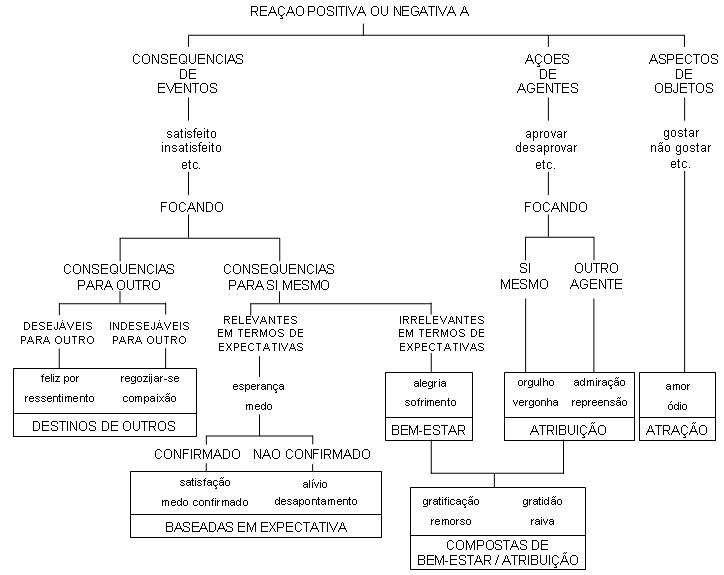
\includegraphics[width=100mm]{figuras/pontarolo_occ.png}
%  \caption{Modelo OCC adaptado de \cite{pontarolo2008modelagem}.}
%  \label{fig:occ_model_original}
%\end{figure*}

A Figura~X\footnote{removido por agora} mostra uma visualização da estrutura
lógica das emoções. As emoções no modelo de \citet{ortony1988cse} já
encontram-se agrupadas em grupos por estarem utilizando regras semelhantes ou
próximas. Esses grupos são representados pelo quadrados e nome do grupo é dado
na parte inferior, assim o ramo de objetos que julga a atração de um indivíduo
com alguma outra coisa (agente ou objeto) possui o grupo de Atração. O ramo de
ações julga a responsabilidade de um agente sobre suas ações e o ramo de
eventos julga a consequência de eventos ou ações desempenhadas. Desse ramo,
o grupo Destinos de outros julga sempre algum outro agente que não é aquele
que esta fazendo a avaliação. Além disso, o grupo denominado Compostas de
Bem-Estar/Atribuição junta os grupos de Bem-Estar (consequência de um evento
sem expectativa) com Atribuição (responsabilidade).

O presente trabalho pretende estudar diferentes ontologias do modelo afetivo
\cite{benta2007ontology,wks2008towards,springerlink:10.1007/978-3-642-01639-448,lera2009semantic}
visando o entendimento destas e suas diferenças. Entretanto, nenhum trabalho propôs
a junção de uma ontologia afetiva com uma humanos virtuais
\cite{Rojas:2006:IRM:1174429.1174442,Gutierrez:2007:OVH:1229160.1229164} com
uma que explique como tratar as percepções do ambiente.


\chapter{Cronograma das atividades}

	\begin{tabular}[c]{c|cccccc}
		Atividades & \begin{sideways} \small{Jul/11} \end{sideways}& \begin{sideways} \small{Ag/11} \end{sideways}& \begin{sideways} \small{S/11} \end{sideways}& \begin{sideways} \small{O/11} \end{sideways}& \begin{sideways} \small{N/11} \end{sideways}& \begin{sideways} \small{D/11} \end{sideways} \\ \hline
		%\cellcolor{gray!50} pendente & \\
		%\cellcolor{green!50} feito & \\
		%\cellcolor{blue!50} andamento & \\
		%\cellcolor{red!85} atrasado &  \\
	Estudo bibliográfico & \cellcolor{gray!50} & \cellcolor{gray!50} & \cellcolor{gray!50} & \cellcolor{gray!50} &  \\
	Elaboração proposta &  & \cellcolor{gray!50} &  &  &  &  \\
	Desenvolvimento da ontologia &  &  & \cellcolor{gray!50} & \cellcolor{gray!50} & \cellcolor{gray!50} &  \\
	Redação da monografia &  & \cellcolor{gray!50} & \cellcolor{gray!50} & \cellcolor{gray!50} & \cellcolor{gray!50} & \cellcolor{gray!50}
	\end{tabular}

\chapter{Estado da Arte} \label{cap:eda}
%2345678901234567890123456789012345678901234567890123456789012345678901234567890

Uma ontologia possui inúmeras utilidades tanto em pesquisa quanto na
indústria. Na pesquisa o foco é uma melhor descrição dos domínio propriamente
dito, enquanto na indústria o foco é a melhor utilização dos recursos de seus
colaboradores. No trabalho de \citet{Gutierrez:2007:OVH:1229160.1229164} existem
excelentes exemplos dos usos possíveis de uma ontologia de humano virtual.
Assim, a primeira seção introduz os modelos psicológicos e explica o modelo de
\citet{ortony1988cse}. Na segunda, apresenta ontologias emocionais
desenvolvidas. A terceira seção descreve os trabalhos com ontologias que visam
descrever o físico ou o mental de um humano virtual.

\section{Modelo Cognitivo Emocional} \label{cap:eda:mce}

Estudos neurológicos recentes \cite{ledoux1998emotional,damasio2004erro}
mostram a importância das emoções na tomada de decisão.
\citet{damasio2004erro} definiu emoção como sendo um estado físico do corpo e
o sentimento sendo a percepção desse estado corporal. Além disso, na psicologia
há diferentes modelos que tentam explicar a afetividade.

\citet{scherer2000tnoe} categorizou esses modelos afetivos em quatro
categorias principais. A primeira categoria, modelos dimensionais, visa
descobrir variáveis que representam eixos das classes emotivas e estabelecem
meios de se mover por esses eixos. Os modelos discretos especificam um
conjunto básico de emoções e especificam regras para que o mecanismo evolua.
Já, a categoria dos baseados em significados se preocupa com as situações
em que o sentimento foi ocasionado e tenta descrever estruturas semânticas dos
mesmos. Por fim, os modelos baseados em componentes entendem que os
sentimentos são aprendidos ao longo do tempo e, sendo assim, estudam o elo
entre os sentimentos e as suas situações. Esse elo é montado de diferentes
formas e varia de pessoa para pessoa.

\begin{figure}[t]
  \centering
    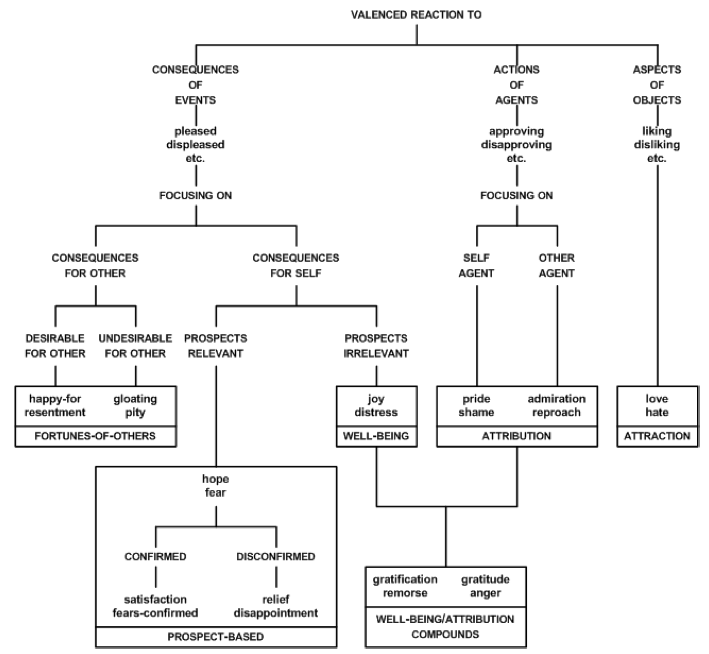
\includegraphics[width=150mm]{figuras/occ.png}
  \caption{Estrutura de emoções \cite{ortony1988cse}.}
  \label{fig:occ_model}
\end{figure}

Um modelo bastante conhecido na Inteligência Artificial foi definido por
\citet{ortony1988cse}. Esse modelo\footnote{A partir daqui o modelo será
referenciado como modelo \occ.} baseado em significados possui 22 emoções
descritas com suas situações. Essas emoções são divididas em
formas de se perceber o mundo a sua volta por consequências (importantes para
alguma meta), ações (julga a responsabilidade) e objetos (atração ou repulsa).
Assim sendo, essas maneiras de se perceber o mundo refletem diferentes jeitos
de se analisar as situações que podem ser relativas aos objetivos, valores
morais ou gostos da pessoa.

A Figura~\ref{fig:occ_model} resume esse modelo e mostra as
percepções possíveis de um indivíduo.  Partindo da direita para esquerda, o
ramo mais básico, \emph{Aspects Of Objects}, é ativado quando se avalia o
gosto de alguém para algum objeto (inanimado ou não). Por exemplo, Millie
gosta de rosas azuis. No seguinte, \emph{Actions Of Agents}, o julgamento das
ações exercidas por outro indivíduo é realizado baseado nos valores morais da
pessoa que está julgando. Exemplo: reprovar a atitude dos bancários que fazem
greve a cada ano. Cabe salientar, que ao julgar ações, o modelo permite um
grau de ``empatia'' chamado pelos autores de ``unidade de força
cognitiva''\footnote{Traduzido literalmente de \emph{Strength of cognitive
unit}.}. Dessa forma, é possível, por exemplo, ficar com orgulho porque uma
atleta ganhou uma medalha ou ficar envergonhado ao descobrir que o vizinho
bate no(s) filho(s).

O último ramo da árvore, mais a esquerda na Figura~\ref{fig:occ_model}, é o
\emph{Consequences Of Events} que representa as coisas que aconteceram (e
foram consideradas importantes), acontecem ou acontecerão (objetivos
almejados)\dev{}. Essas emoções são avaliadas segundo as suas consequências
para o alcance ou impedimento dos seus objetivos. A emoção sentida ao receber
uma boa nota em um teste ou a de não chegar em um destino planejado são
exemplos possíveis desse ramo do modelo.

Toda a emoção do modelo trabalha com duas intensidades. A intensidade da
emoção que representa o físico e a intensidade do sentimento que representa o
quanto o agente esta percebendo daquela emoção. Dessa forma, um indivíduo só
possui sentimento quando a intensidade da emoção ultrapassa um
determinado limite\dev{}.  Essa intensidade é obtida por uma função matemática
que utiliza variáveis de dois tipos: local, que influência as emoções do ramo
específico; e global, que influência todas as emoções do modelo.  Um exemplo
de variável local é o desejo, enquanto que um exemplo de variável global pode
ser o senso de realidade de uma pessoa.

\citet{bates1994role} foi um dos primeiros a trabalhar na utilização de emoções
na na área de animação. Nessa área, o estudo do comportamento humano é
realizado visando imitar as ações humanas. A principal afirmativa do trabalho
é que o comportamento emotivo de um personagem é um papel importante para que
o mesmo pareça ter vida própria. Esse trabalho utilizou o modelo descrito
visando melhorar a credibilidade de seus atores. Por exemplo, um dos agentes
lida com o medo sendo agressivo com os outros enquanto outro agente lida com a
mesma emoção sendo retraído.

Visando entender melhor o impacto da emoção na tomada de decisão,
\citet{zhang2009emotional} desenvolveram uma aplicação que os sentimentos
afetam o planejamento das ações à serem realizadas.
\citet{neto2010construction} focaram no mesmo objetivo, porém foco do estudo
foi o impacto da memória no planejamento. Sendo assim, eles fizeram um meio
para o agente ``esquecer'' determinadas crenças quando o estado emocional
fosse diferente daquele guardado anteriormente. Essa característica torna o
planejamento e as atitudes dos personagens virtuais mais realistas.

O projeto \emph{Relational Agents} de \citet{bick2003relational} possui o
objetivo de possibilitar aos usuários a criação de um relacionamento social e
emocional com longa duração. Com a confiança no agente se torna possível
discutir tarefas mais importantes como melhora da saúde ou até a compra de uma
casa \cite{bickmore2009virtual}. Da mesma forma, o projeto AIDA\footnote{Mais
detalhes, ver \url{http://senseable.mit.edu/aida}.} tem por objetivo entender
o estado afetivo da pessoa dirigindo para tentar sugerir ao usuário mudanças
em suas rotas baseado na rotina aprendida anteriormente. Ambos os trabalhos
podem ser entendidos como enquadrados na área de IHC.

Um dos trabalhos mais conhecidos utilizando o modelo \occ é, sem dúvida, o de
\citet{kshirsagar2002multilayer}\todo{falar mais na dissertacao}. Ele utilizou
as emoções levantadas no modelo em conjunto com um modelo de personalidade
baseado na psicologia que leva em consideração 5 fatores. O primeiro fator,
extroversão, é descrito como a preferência para o comportamento em situações
sociais. O segundo, agradabilidade, é a interação com outros outros
indivíduos. Outro fator é a conscientização que é a organização e persistência
das metas. A tendência de pensamentos negativos é o chamada de fator
neurótico. O último fator é o que descreve se a pessoa tem interesse em
cultura ou é ``cabeça aberta''.

\section{Ontologias Emocionais} \label{cap:eda:oe}

Ontologias emocionais visam descrever emoções ou aspectos afetivos de um
indivíduo se baseando ou não em estudos da psicologia. Em
\citet{benta2007ontology} foi feita a construção de uma ontologia escrita em
\OWL. Nesse trabalho as emoções são divididas em primárias e secundárias, as
secundárias se originam a partir das primárias. As emoções primárias ou
básicas, não cognitivas, são: \emph{Angry}, \emph{Disgust}, \emph{Fear},
\emph{Happy}, \emph{Neutral}, \emph{Sad} e \emph{Surprise}. As emoções
secundárias, cognitivas, descritas são ao todo 4. O interessante aqui é que
essas 4 emoções são inferidas a partir de propriedades de objeto. Além disso,
há o conceito de emoção ativa que é a emoção predominante naquele momento. O
valor da emoção é calculado da seguinte forma, a sensibilidade (predisposição
a emoção varia de 0 à 1) multiplicado pela intensidade da emoção. A emoção
predominante é o maior valor entre as emoções.

No modelo definido por \citet{ortony1988cse} a distinção entre os tipos de
emoções não existe porque se pressupõe que toda emoção exige um certo nível de
cognição. Também, não existe um limite no que pode ou não ser percebido em
quantidade de emoções, mas sim no que se esta sendo perseguido como meta. Fora
isso, se pode pensar que emoções opostas compartilham os mesmos atributos e,
por isso, essas emoções não serão sentidas ao mesmo tempo.

Não tendo nenhuma informação de uma teoria de emoções específicas modeladas em
sua ontologia, \citet{wks2008towards} criou uma ontologia de alto nível se
aproveitando de outra ontologia de alto nível e de uma de analise léxica. O
principal conceito da ontologia pode ser pensado como o de sensores que são
objetos físicos que recebem informações do ambiente e as ``transportam'' para
o mundo mental. Sendo assim, é possível reconhecer a percepção recebida
utilizando a memória e descrever a nova situação. Todavia, o presente trabalho
não tem objetivo de ser uma ontologia de alto nível\dev{}.

\citet{springerlink:10.1007/978-3-642-01639-448} desenvolveram um motor de
emoções que utiliza um modelo de mistura de emoções em conjunto com o modelo
\occ. O trabalho deles dividiu o modelo em camadas, nas quais cada camada tem
uma responsabilidade distinta e que visa complementar a anterior. A
camada de classificação visa determinar que categoria ou ramo será afetado. A
seguinte de quantificação determina a intensidade da emoção. A de interação
analisa os efeitos nas categorias emocionais do personagem. A próxima mapeia
as 22 emoções do modelo para pelo menos uma expressão e a última camada é a
responsável por realizar a expressão propriamente dita no ator.

Esse trabalho ainda utilizou um modelo dimensional para misturar as emoções
primárias. Assim, as emoções secundárias podem ser descobertas a partir do
nível dos eixos afetados. O trabalho mostra quase todas as emoções do
ramo de consequência de eventos, com exceção das emoções de \emph{Hope} e
\emph{Fear}. As emoções do modelo \occ são consideradas as
emoções primárias e como secundárias estão as emoções construídas a partir da
mistura de outras emoções. Como dito anteriormente, estaria incorreto fazer
essa diferenciação no modelo sendo proposto porque ela não é realizada no
modelo \occ original.

Um modelo genérico que representa o ambiente e eventos que estão envolta de um
personagem, sua personalidade e preferencias foi feito por
\citet{lera2009semantic}. Nesse trabalho o foco eram emoções que podem ser
representadas no rosto. Assim, a identificação do contexto através de eventos
e do retorno afetivo. Além disso, as expressões faciais são modificadas
dependendo dos eventos do ambiente e, também, da personalidade, metas e
preferências dos atores virtuais.

\citet{adam2009alfototoe} formalizaram o modelo \occ de maneira lógica. A
formalização construída possui algumas limitações, por exemplo a probabilidade
de eventos é medida de forma comparativa, isto é, o evento A é mais provável
que o evento B. Além disso, a foi necessário estabelecer uma ordem temporal
das ações sendo desempenhadas.  Entretanto, o autor propõem uma diferenciação
entre ação e evento. O primeiro é causado intencionalmente pelo agente\dev{},
enquanto o segundo o agente não tem controle da ação. Por exemplo, o ato de
espirrar seria um evento.

\section{Ontologias de Humanos Virtuais} \label{cap:eda:odhv}

A primeira ontologia a ser abordada foi apresentada durante a introdução do
UEM no trabalho de \citet{paiva2005ontology}. Ela descreve o comportamento
habitual de atores em uma cidade virtual. Desse modo, os atores possuem
lugares que se dirigem rotineiramente e eventualmente. Por exemplo, um local
rotineiro é onde se trabalha e um local eventual pode ser à igreja.

Na Figura~\ref{fig:UEM}\footnote{As relações de generalização possuem a mesma
semântica que na UML, as relações direcionais são relações binárias entre as
instâncias das classes.} pode ser observado 5 conceitos principais, o primeiro
\emph{Agent} se relaciona com o conceito \emph{Profile} para determinar o tipo
de agente. O \emph{Profile} do agente pode variar entre \emph{Unemployed Adult},
\emph{Employed Adult}, \emph{Child} e \emph{Dependent}. Os tipos \emph{Child}
e \emph{Employed Adult} possuem destinos fixos em determinados momentos do dia
e, depois, destinos randômicos. \emph{Unemployed Adult} só possui destinos
randômicos e \emph{Dependent} necessita de um adulto para se mover.

\begin{figure}[t]
  \centering
    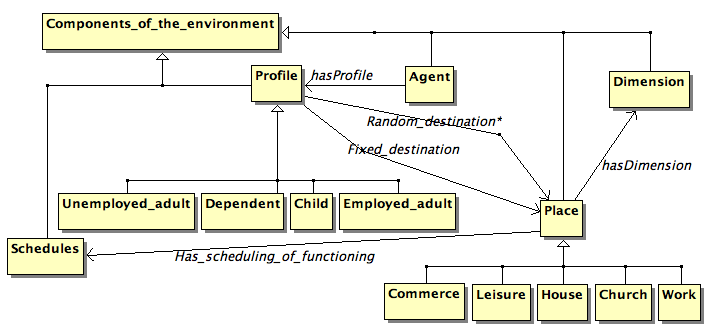
\includegraphics[width=150mm]{figuras/UEMontology.png}
  \caption{Modelo de ambiente urbano \cite{paiva2005ontology}.}
  \label{fig:UEM}
\end{figure}

Assim, \emph{Profile} permite definir locais usuais (fixos) e eventuais
(randômicos). Esses locais são definidos pelo conceito \emph{Place} que contêm
uma descrição de sua capacidade (quantidade máxima de atores), dimensão
(acessível por relação) e horário de funcionamento (acessível por relação). O
conceito de \emph{Dimension} guarda a posição dos eixos X e Y, altura e
largura. Finalmente, o último \emph{Schedules} possui o horário de abertura e
fechamento, intervalo de entrada e tempo médio de permanência. %A decisão de
%para onde determinado agente irá é feita pelo ambiente através do conhecimento
%do perfil do ator, dessa forma, é possível carregar uma maior quantidade de
%atores.

Este trabalho pode ser pensado como a descrição da mentalidade dos personagens
através da descrição dos atores em um ambiente urbano em sua vida normal. O
foco da ontologia seguinte é o humano virtual propriamente dito. Assim, as
informações gerais do personagem, como, por exemplo, raça, cor e outros são
armazenadas na ontologia descrita visando uma descrição completa e reusável.
A Figura~\ref{fig:OVH} apresenta os principais conceitos da ontologia
desenvolvida por \citet{Gutierrez:2007:OVH:1229160.1229164}.

O conceito principal definido na ontologia é o \emph{Virtual Human}. O modelo
pode ser utilizado para representar pessoas virtuais ou reais. Humanos
(virtuais) podem serem descritos por \emph{Structural Descriptors} e
\emph{Morphological Descriptors}. Neste último são guardados os dados gerais
do personagem, por exemplo idade, sexo, altura, peso e etc. No outro conceito,
\emph{Structural Descriptors} é uma abstração que define os pontos de entrada
para uma variedade de descritores\todo{descritores que descrevem soa estranho} que descrevem a organização do humano
virtual. No modelo o foco foi organização por esqueleto e se baseando na
especificação H-Anim\footnote{É uma especificação que descreve quantidade,
posição e rotação dos ossos para tentar padronizar os modelos.
Veja \url{http://www.h-anim.org/}.} e como pode ser visto é possível guardar
informações de geometria, textura e outras informações.

\begin{figure}[t]
  \centering
    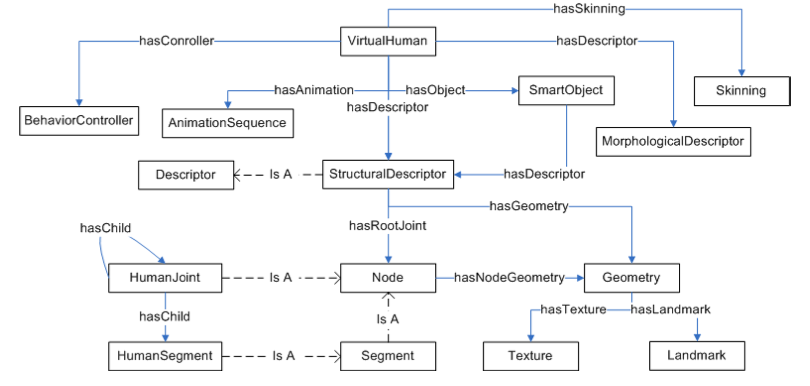
\includegraphics[width=150mm]{figuras/gutierrezVH.png}
  \caption{Ontologia de Humano Virtual \cite{Gutierrez:2007:OVH:1229160.1229164}.}
  \label{fig:OVH}
\end{figure}

Assim, o corpo humano consiste de um número de \emph{Segment} (por exemplo,
pé, mão e etc) que são conectados por \emph{Node}. Cada \emph{Node} pode
conter outros e, também, um \emph{Segment}. Além disso, ela pode ser animada
de duas formas. A primeira é através de uma animação sequencial pre-gravada
representada pelo conceito \emph{Animation Sequence} e a segunda é utilizando
o conceito de \emph{Behavioral Controller}. Esse último pode ser utilizado
para embutir um comportamento mais autônomo. Por fim, o conceito de
\emph{Smart Object} representa todos os objetos que podem ser manipulados por
um humano virtual.

\citet{grimaldo2006ontology} descreveu uma ontologia de ambiente inteligente
onde os agentes podem interagir, isto é, descreve o ambiente e permite
obter o estado do mundo. Por exemplo, a garrafa esta sobre a mesa ou o copo é
segurado pelo garçom. Além disso, em \citet{muller2010amabid} foi feita uma
ontologia para descrever atores implementados em \jason\footnote{Ver
\url{http://jason.sf.net} para mais detalhes.} de uma visão literária. Ambos
os trabalhos possuem uma visão simplificada dos atores por não serem o foco
principal de seus trabalhos.

%2345678901234567890123456789012345678901234567890123456789012345678901234567890

\chapter{Trabalho Proposto} \label{cap:tp}
%2345678901234567890123456789012345678901234567890123456789012345678901234567890

O trabalho visa o desenvolvimento de uma ontologia que englobe o modelo
psicológico de emoções explicado na seção~\ref{cap:eda:mce}, uma ontologia de
humanos virtuais e uma de percepção. A criação das ontologias que, além de
fazerem o raciocínio, definem um vocabulário básico a ser conhecido e, dessa
forma, torna a configuração mais fácil para o leigo. Por exemplo, um
desenvolvedor só precisa conhecer a ontologia de percepção proposta para
saber\dev{} o que o agente deve enviar de crenças ou percepções e o que
esperar em retorno.

%% Reescrito acima
%O trabalho visa dois objetivos principais: (i) apoiar o desenvolvimento de
%aplicações; (ii) minimizar a dificuldade de configuração existente. O primeiro
%objetivo é alcançado com a construção de artefatos de software que leem e
%questionam as ontologias via Jason. O segundo objetivo é alcançado pela
%criação das ontologias que, além de fazerem o raciocínio, definem um
%vocabulário básico a ser conhecido. Por exemplo, um desenvolvedor só
%precisa conhecer a ontologia de percepção proposta para saber\dev{} o que o agente
%deve enviar de crenças ou percepções e o que esperar em retorno.

A seção~\ref{cap:tp:oa} descreve a ontologia afetiva desenvolvida. A descrição
de como a ontologia de humano virtual foi realizada esta explicada na
seção~\ref{cap:tp:ruodhv}. Na seguinte, a ontologia de percepção é detalhada.
%seção~\ref{cap:tp:odp}
Por fim, a seção~\ref{cap:tp:cdu} demostra a utilização da ontologia final.

\section{Ontologia Afetiva} \label{cap:tp:oa}

A fundamentação do modelo afetivo sendo utilizado aqui é o proposto por
\citet{ortony1988cse} e encontra-se explicado na seção \ref{cap:eda:mce}. A
ontologia proposta tinha como ideia inicial não utilizar regras, porém como
pode ser observado na Tabela~\ref{tab:oa:geral} foi necessário a criação de
regras para suportar o raciocínio no nível de indivíduo corretamente. As
regras que ajudam a conclusão das relações \emph{hasKnow}, \emph{hasFriend} e
\emph{hasEnemy} são diferentes das demais por causa que elas tem como
característica operar no domínio e na imagem da classe \emph{Agent}. Por
exemplo, se John avalia que se relaciona bem com Jose então John tem amigo
Jose. Note que o contrario não é necessariamente verdade, o Jose pode apenas
saber que conhece o John.

\begin{table}
	\caption{Ontologia proposta com expressividade: ALCHIN(D).}
	\label{tab:oa:geral}
	\begin{center}
	\begin{tabular}{|c|c|}
	%\begin{tabular}{|p{34mm}|p{50mm}|p{50mm}|}
		\hline
		Descrição & Quantidade \\ \hline
		Classes &  45 		\\ \hline
		Propriedade de Objetos & 16 \\ \hline
		Propriedade de Dados & 14 \\ \hline
		Indivíduos &  0		\\ \hline
		Regras & 7 \\ \hline
	\end{tabular}
	\end{center}
\end{table}

Na Figura~\ref{fig:rlocc} são mostradas as regras desenvolvidas, elas dependem
que os indivíduos da ontologia sejam marcados como diferentes um do outro.
Assim, recomenda-se fortemente que quando registrar um indivíduo da classe
\emph{Object} ou \emph{Agent} que a informação de igualdade ou diferenciação
seja preenchida\dev{}. Assim, se evita que o raciocinador conclua que não
conhece a resposta e chegue a uma conclusão não esperada.

\begin{figure}[t]
  \centering
  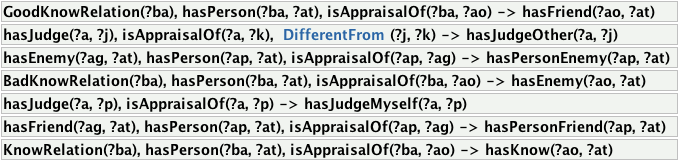
\includegraphics[width=14cm]{figuras/rules-LOCC.png}
  \caption{Regras da ontologia proposta.}
  \label{fig:rlocc}
\end{figure}

A Figura~\ref{fig:kplocc} mostra a árvore de relações que tem como imagem
dados ou instâncias (objetos). Ao olhar se comparar as Figuras~\ref{fig:rlocc}
e Figura~\ref{fig:kplocc} se chega a conclusão que as propriedades que as
regras concluem não precisam ser configuradas pelo usuário. Assim, ao invés de
16 propriedades de objetos conforme informado na Tabela~\ref{tab:oa:geral}
apenas 9 precisam ser conhecidas. Dessas a propriedade mais utilizada é a
\emph{hasSomething} que serve para indicar o que esta sendo avaliado. Note que
\emph{hasPerson} deve ser usado quando o indivíduo em avaliação for um membro
da classe \emph{Agent}. Já, a relação \emph{hasJudge} serve para indicar que o
membro da classe \emph{Object} esta sendo avaliado. Por exemplo, Millie tem
uma avaliação de julgando seu carro com uma valoração positiva.

\begin{figure}[b]
  \centering
  \begin{tabular}{cc}
  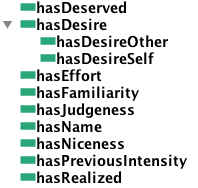
\includegraphics[height=4cm]{figuras/dataProperty-LOCC.png} & 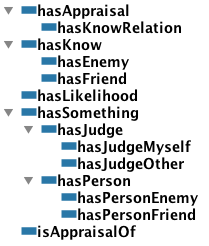
\includegraphics[height=5cm]{figuras/objectProperty-LOCC.png} \\
  (i) Relações de dados & (ii) Relações de Objetos
  \end{tabular}
  \caption{As relações existentes na ontologia proposta.}
  \label{fig:kplocc}
\end{figure}

Todos os dados numéricos da ontologia são inteiros. Isso foi feito com a
finalidade de permitir que o usuário normalize\dev{} o número obtido da
maneira que desejar. Além disso, foi tomada a decisão de não especificar o
domínio da maioria das propriedades por causa que isso forçaria um
enquadramento em classes não desejadas. Por exemplo, se a relação
\emph{hasLikelihood} tiver o domínio \emph{ConsequenceForSelf} e existir
indivíduo com somente essa relação então o mesmo seria enquadrado no conceito
\emph{ConsequenceForSelf}. O correto nesse caso seria não ser concluído nada,
isto é, pertencer à classe \emph{Thing}.

A estrutura da ontologia pode ser visualizada na Figura~\ref{fig:tlocc}. Além
disso, pode ser recomendável olhar a
Figura~\ref{fig:occ_model}~(pg.~\pageref{fig:occ_model}) do modelo criado por
\citet{ortony1988cse} durante o resto da discussão dessa seção. Os
sub-conceitos de \emph{Emotion} correspondem aos ramos do modelo original. O
ramo \emph{ActionsOfAgents} julga a responsabilidade e o quanto o agente que
realizou uma ação ou evento se desviou do esperado, o de
\emph{ConsequencesOfEvents} julga a consequência de um evento e
\emph{AspectsOfObjects} julga a atração para com um objeto.

O primeiro ramo a ser abordado é, o menos cognitivo, \emph{AspectsOfObjects}.
As emoções desse tipo são relacionadas com atratividade e familiaridade.
Entretanto, essas duas relações foram consideradas equivalentes porque o
importante, para o modelo, é quando ambas são positivas ou ambas negativas.
Assim sendo, uma pode assumir os dois papeis sem maiores penalidades e
simplificando a modelagem. A emoção \emph{Hate} é modelada como tendo a
propriedade de familiaridade (\emph{hasFamiliarity}) com valores negativos,
enquanto a emoção \emph{Love} tem valoração dessa mesma propriedade positiva.
Caso o valor seja zero, nada pode ser concluído.

\begin{wrapfigure}{r}{0.4\textwidth}
  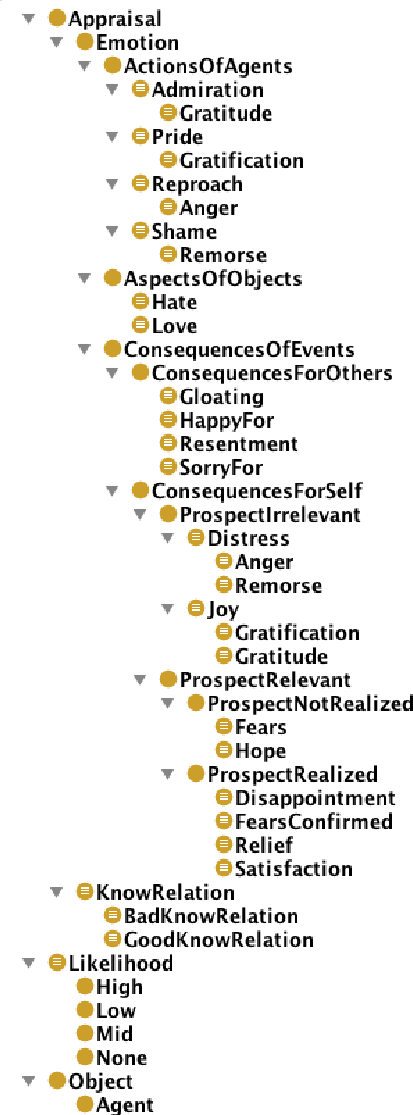
\includegraphics[height=16cm]{figuras/hierarquiaLOCC.png}
  \caption{Taxonomia da ontologia proposta baseado no modelo.}
  \label{fig:tlocc}
\end{wrapfigure}

Cabe notar que parece estranho uma emoção \emph{Love} com um objeto, porém
essa emoção foi escolhida por quem montou o modelo por ser a emoção mais forte
de seu tipo. Assim, níveis menores implicam em outros tipos de emoção. Além
disso, conforme explicado no trabalho, agentes podem ser vistos como objetos
quando se esta avaliando a sua atração. Assim, todo agente (\emph{Agent}) é um
objeto (\emph{Object}). Por exemplo, John esta apaixonado pela Millie ou
John tem repulsa por televisão.

O segundo conceito chamado \emph{ActionsOfAgents}, ele pode ser pensado como
um ramo que julga a responsabilidade por uma determinada ação ou evento.
Assim, esse ramo é capaz de gerar emoções de: Admiração (\emph{Admiration}),
Orgulho (\emph{Pride}), Vergonha (\emph{Shame}) e Reprovação
(\emph{Reproach}). Por exemplo, Jose possui orgulho (por cozinhar) ou Dilu
reprova Jose (porque ele come carne).

Na definição, as emoções de orgulho e vergonha podem acontecer mesmo quando se
esta avaliando ações de outras pessoas. Por exemplo, Dolores tem vergonha de
sua mãe (que não cozinha). Essa conclusão é possível por causa de uma relação
que ele propõem de empatia. Como em nenhum momento da definição, ele dá mais
detalhes dessa empatia resolveu-se considerar que vergonha e orgulho são
emoções sentidas somente quando o agente esta avaliando a si mesmo e, dessa
forma, o exemplo anterior não é possível.

As emoções que julgam responsabilidade são definidas como tendo uma relação de
julgamento (\emph{hasJudge}) e uma relação que mapeia o valor do julgamento
(\emph{hasJudgeness}) que representa o quanto o agente se desviou do
comportamento esperado, isto é, em casos de aprovação é um valor positivo e em
casos de reprovação é um valor negativo. Todavia, isso ainda não permite
diferenciar a emoção de admiração da emoção de orgulho ou a reprovação da de
vergonha. Essa distinção é possível ao se dividir a relação de julgamento com
duas sub-relações: tem auto-julgamento (\emph{hasJudgeMyself}) e tem
julgamento de outro (\emph{hasJudgeOther}).

A utilização de sub-propriedade torna possível escrever a ontologia da maneira
esperada suprindo o problema. Entretanto, para o usuário pode se tornar
complicado ter que lembrar quando utilizar uma sub-propriedade ou outra.
Assim, foi resolvido deixar o usuário sempre utilizar a relação de julgamento
(\emph{hasJudge}) e via 2 regras inferir se é um auto-julgamento ou o
julgamento de outra pessoa. Para essas regras funcionarem da maneira correta,
o usuário deve declarar que os agentes ou objetos são diferentes. Caso isso
não ocorra, o sistema considera que não há informação para verificar se um
individuo é igual ou diferente que o outro e concluir que não conhece a
resposta. Além disso, a relação de julgamento tem como imagem o conceito
\emph{Object}. Dessa forma, os exemplos anteriores são todos válidos.

Cabe salientar que toda avaliação tem pelo menos duas relações. A primeira
relação serve para conhecer quem esta avaliando (\emph{isAppraisalOf}) e a
outra serve para indicar quem ou o que esta sendo avaliado
(\emph{hasSomething}). Em muitas avaliações essa última pode não ser
informada sem nenhum prejuízo. O último ramo, chamado de
\emph{ConsequencesOfEvents} é dividido em: \emph{ConsequencesForSelf} e
\emph{ConsequencesForOthers}. Toda essa divisão foca na consequência de um
evento ou ação realizado por um determinado agente. Por exemplo, Dilu tem pena
de Jose, Jose tem esperança (de ser promovido), John tem satisfação (por
estar almoçando) ou Millie esta alegre (por cozinhar).

A \emph{ConsequencesForOthers} expressa 4 emoções: \emph{HappyFor},
\emph{SorryFor}, \emph{Gloating} e \emph{Resentment}. Na definição, essas
emoções dependem: do grau de desejabilidade nosso para com o outro; do grau de
desejabilidade que se presume que o outro tenha; do grau de merecimento do
evento; do tipo de relacionamento com a pessoa. Na ontologia proposta, a principal
diferença com o modelo original é que foi considerado que o grau de
desejabilidade nosso para com o outro e o grau de merecimento do evento são os
mesmos. Dessa forma, se pode utilizar apenas três relações para descrever as
4 emoções.

A relação de merecimento (\emph{hasDeserved}) e relação de desejabilidade
presumida (\emph{hasDesireOther}) são avaliadas de acordo com sua valoração
positiva ou negativa. A terceira relação é a que liga o outro individuo/agente
(\emph{hasPerson}) sendo avaliado. Para se ter o conhecimento de quem esta
julgando é uma pessoa amiga (\emph{GoodKnowRelation}) ou inimiga
(\emph{BadKnowRelation}), esses conceitos foram criados e precisam ser
configurados para cada um dos agentes em questão. O agente pode declarar que
só conhece uma pessoa, que conhece e é um amigo ou que conhece e não gosta
dela (inimiga). Entretanto, quem precisa dessa informação é o conceito de
avaliação quando as relações \emph{hasPersonEnemy} e \emph{hasPersonFriend}
precisam ser descobertas.

\emph{ConsequencesForSelf} se divide entre consequências de eventos com
probabilidade relevante (\emph{ProspectRelevant}) e irrelevante
(\emph{ProspectIrrelevant}). Cabe salientar que esses dois conceitos se
relacionam com probabilidade (\emph{hasLikelihood}), entretanto enquanto o
primeiro conceito se relaciona com a parte não nula. A outra se relaciona
somente com essa. Dessa forma, ambos os conceitos são disjuntos. A classe de
probabilidade relevante pode ser dividida ainda entre possibilidade não
realizada (\emph{ProspectNotRealized}) e realizada (\emph{ProspectRealized}).

As emoções \emph{Hope} e \emph{Fear} fazem parte do conceito
\emph{ProspectNotRealized}. Esse conceito usa as relações \emph{hasLikelihood}
e \emph{hasDesireSelf}. Essa última propriedade é um número que
representa o desejo de se obter ou repudiar o evento. Além disso, quando o
evento ocorre a emoção atual pode virar uma emoção do conceito
\emph{ProspectRealized}, isto é, \emph{Fear} pode virar ou
\emph{FearsConfirmed} ou \emph{Relief} e \emph{Hope} pode virar ou
\emph{Satisfaction} ou \emph{Disappointment}.

O conceito \emph{ProspectRealized} não se relaciona em nenhum momento com a
relação \emph{hasLikelihood} porque o evento já aconteceu ou não vai mais
acontecer. Assim, ele possui três relações distintas das anteriores, a
primeira é o grau de realização de um evento (\emph{hasRealized}), isto é, a
visão do agente sobre como a consequência do evento aconteceu. A segunda
relação \emph{hasPreviousIntensity} recebe a valoração da emoção de medo ou
esperança do evento que tinha probabilidade e serve para saber se o evento é
um evento bom (esperança) ou ruim (medo). Já, a terceira \emph{hasEffort}
tenta estimar o grau de esforço que foi dispendido para a atração ou repulsa
da consequência do evento.

O conceito \emph{ProspectIrrelevant} é parecido com o conceito
\emph{ProspectRelevant} com a diferença que a relação \emph{hasLikelihood} vai
somente para valores nulos. Alem disso, as emoções desse conceito e do
\emph{ActionsOfAgents} podem ser misturadas formando um conceito de composto.
A composição é quando uma emoção pode ser encaixada em mais de uma emoção
como no caso de se estar alegre (\emph{Joy}), orgulhoso (\emph{Pride}) e
gratificado (\emph{Gratification}). Por fim, o conceito \emph{Setup}
\todo{na dissertacao falar mais sobre isso} é o utilizado para manter junto da
ontologia criada o limite mínimo para uma emoção virar sentimento\dev{}. Ele é
melhor explicado na seção~\ref{cap:tp:cdu}~(pg.~\pageref{cap:tp:cdu}).

%a transferencia eh feita pelo sistema;
%os dados sao carregados para memoria e eliminados;
%conforme reparado nao ha decaimento da emocao, a mesma eh instantanea;
%2345678901234567890123456789012345678901234567890123456789012345678901234567890

\section{Reutilizando uma ontologia de Humanos Virtuais} \label{cap:tp:ruodhv}

Na seção~\ref{cap:eda:odhv} foi explicado a ontologia de
\citet{Gutierrez:2007:OVH:1229160.1229164} que descreve humanos virtuais de
uma maneira bem detalhada. Entretanto, a nossa intenção no presente trabalho é
focado no comportamento do personagem. Dessa forma, a ontologia que será
utilizada é a de \citet{paiva2005ontology} que descreve uma vida normal.

\begin{figure}[t]
  \centering
    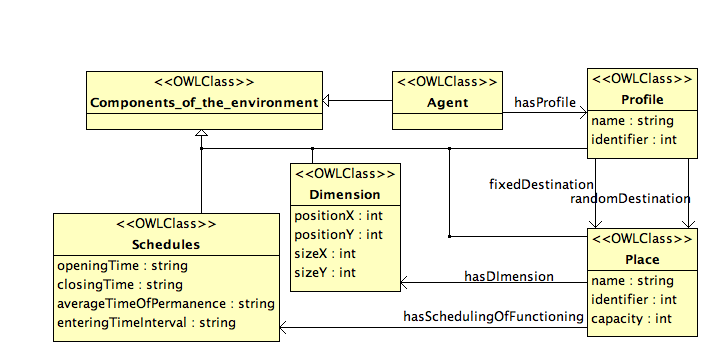
\includegraphics[width=150mm]{figuras/uem-tbox.png}
  \caption{T-Box baseado no modelo de ambiente urbano \cite{paiva2005ontology}.}
  \label{fig:UEM:TBOX}
\end{figure}

A Figura~\ref{fig:UEM:TBOX} demostra a ontologia que será utilizada, como é
possível observar as subclasses dos conceitos \emph{Profile} e \emph{Place}
foram removidas\footnote{Compare a Figura~\ref{fig:UEM:TBOX} com a
Figura~\ref{fig:UEM} da página~\pageref{fig:UEM}.} por serem consideradas parte
da A-Box. Além disso, o conceito \emph{Components\_of\_the\_environments} esta
sendo pensando como um sub-conceito do conceito \emph{Setup} na nossa
ontologia por causa que esse representa configurações gerais.

Essas configurações gerais são carregadas, normalmente, em outras partes do
sistemas e então eliminadas por causa que elas não influenciam as emoções
diretamente. Fora isso, foi introduzido uma nova relação chamada
\emph{hasCharacter} que mapeia o conceito de agente da seção anterior para o
conceito utilizado no trabalho de \citet{paiva2005ontology}. Dessa forma, um
agente na ontologia do modelo \occ pode descobrir seu perfil e descobrir seus
locais visitados regularmente.

% eu nao tenho certeza sobre isso, porem seria interessante ter uma relacao
% hasDimension da Object para Dimension. Dessa forma um objeto teria
% conhecimento mesmo que abstrato sobre suas dimensões para o caso de ser
% necessario fazer a bounding box collission...

\section{Ontologias de Percepções} \label{cap:tp:odp}
% de percepcoes virou do ambiente
% voltou a ser de percepcoes

\citet{doyle1998annotated} propuseram que o mundo contivesse uma serie de
anotações nos objetos. Assim, o agente poderia conhecer apenas a forma de
questionar os objetos sobre suas formas de usar, suas descrições e suas outras
características. Esse conceito veio do conceito \emph{affordance} que
propriedades de um objeto determinam como ele será usado. Dessa forma, uma
cadeira tem a propriedade de ser sentada e uma porta tem as propriedades de
ser aberta ou ser fechada.

Nesse trabalho foi usado 5 tipos de anotações: (i) anotações emocionais,
explicam como um agente responde ``emocionalmente''; (ii) anotações de
resposta, explicam como o agente deve reagir ao evento no ambiente pode ser
uma ação especifica ou uma sugestão de crença; (iii) anotações de resolução de
problemas, descreve o estado do problema  e permite anotar dicas que o agente
talvez fale ou realize; (iv) anotações de papel, informam o agente sobre ações
relevantes para determinados trabalhos no mundo; (v) anotações de jogo,
descreve o estado do jogo permitindo sugerir movimentos.

\citet{kallmann1999modeling} explicaram uma ideia similar, os objetos no mundo
são os responsáveis por proverem para o personagem o como ele deve ser usado.
Durante a animação do personagem estar abrindo a porta, por exemplo, quem esta
no controle do mesmo é o ``agente'' que controla a porta porque o agente do
personagem delega para o da porta realizar a sua animação. Dessa forma,
esses objetos inteligentes precisam ter um determinado nível de conhecimento
sobre o personagem.

De uma maneira similar, o conceito de artefatos que possuem propriedades
observáveis e utilizáveis foi criado por \citet{ricci31cartago}. Por exemplo,
uma porta pode ter como propriedade observável se ela esta aberta ou fechada e
como propriedade utilizável ou ação possível ela ser aberta ou ser fechada.
Essas ações podem ficar disponíveis conforme o estado atual do objeto, mas o
controle da disponibilidade é do próprio objeto por que é ele que sabe como
realizar a ação propriamente dita. O agente unicamente diz de alguma forma que
o objeto tem que realizar tal ação. Nesse trabalho, não é mencionado que o
agente que controla o personagem delega sua animação para o objeto.

Assim, ...


%... Última coisa
%
%Uma ontologia de percepção esta ligada a formas de perceber o ambiente, por
%isso foi estudado o \emph{CArtAgO}\cite{ricci31cartago} e o
%\emph{EIS}\cite{behrens2009taeisfaop}. Todavia, em um estudo preliminar sobre
%esses trabalhos foi visto que o foco aqui não é a descrição do ambiente em si
%e, sim, como o agente interpreta essas informações que viram de maneira
%anotada nas percepções\dev{}.

\section{Caso de uso} \label{cap:tp:cdu}

Ok, eu sei o que eh.
Mas, como eu faco funcioanr?
... tem que tomar o conceito Setup para melhor explicar ele!

Thunder, thunder, thundercats, Ho! Thundercats are on the move, Thundercats are loose. Feel the magic, hear the roar, Thundercats are loose. Thunder, thunder, thunder, Thundercats! Thunder, thunder, thunder, Thundercats! Thunder, thunder, thunder, Thundercats! Thunder, thunder, thunder, Thundercats! Thundercats!

Knight Rider, a shadowy flight into the dangerous world of a man who does not exist. Michael Knight, a young loner on a crusade to champion the cause of the innocent, the helpless in a world of criminals who operate above the law.

80 days around the world, we'll find a pot of gold just sitting where the rainbow's ending. Time - we'll fight against the time, and we'll fly on the white wings of the wind. 80 days around the world, no we won't say a word before the ship is really back. Round, round, all around the world. Round, all around the world. Round, all around the world. Round, all around the world.

Hong Kong Phooey, number one super guy. Hong Kong Phooey, quicker than the human eye. He's got style, a groovy style, and a car that just won't stop. When the going gets tough, he's really rough, with a Hong Kong Phooey chop (Hi-Ya!). Hong Kong Phooey, number one super guy. Hong Kong Phooey, quicker than the human eye. Hong Kong Phooey, he's fan-riffic!

Mutley, you snickering, floppy eared hound. When courage is needed, you're never around. Those medals you wear on your moth-eaten chest should be there for bungling at which you are best. So, stop that pigeon, stop that pigeon, stop that pigeon, stop that pigeon, stop that pigeon, stop that pigeon, stop that pigeon. Howwww! Nab him, jab him, tab him, grab him, stop that pigeon now.


\chapter{Considerações finais}

O presente artigo visa apresentar uma visão do trabalho que está sendo feito
para a construção de um simulador no qual os atores e ambientes interagem.
Entretanto, a ontologia foi omitida porque está ainda sendo aprimorada.  A
idéia apresentada não é nova, porém, o ponto chave é a ontologia permitir aos
agentes raciocinarem sobre suas emoções de forma transparente.  Essa
transparência é útil porque permite ao animador conhecer e, até mesmo,
especificar o personagem com um grau bastante elevado de abstração.
%
Dessa forma, dois agentes com a mesma especificação, ao enfrentarem a mesma
situação, terão o mesmo comportamento quando tiverem vivenciado as mesmas
experiências. Essa experiência inclui as informações adquiridas sobre o
ambiente e sobre os demais atores e não somente os interesses e metas do
mesmo.

O modelo OCC em uso no presente trabalho, foi definido em
\citeyear{ortony1988cse} e possui ao todo 22 emoções especificadas por regras
que demonstram quando a mesma acontece. Entretanto, em nenhum momento da sua
definição foi tratado explicitamente como uma emoção afeta as outras presentes
no personagem.
%
A ferramenta em desenvolvimento tem como interesse a simulação computacional
do comportamento humano e, dessa forma, ela pode ser utilizada de diferentes
maneiras e pode coletar diferentes informações para análises com diversos
propósitos.

\chapter{remover no release}
     \begingroup
     \parindent 0pt
     \parskip 2ex
     \def\enotesize{\normalsize}
     \theendnotes
     \endgroup


%\bibliographystyle{abnt-alf}
\bibliography{mestrado}

	\vfill

%   \begin{center}
%		\rule{8cm}{.1mm} \\ Orientador: Prof.~Dr.~Rafael Heitor Bordini
%    \end{center}
%   \begin{center}
%		\rule{6cm}{.1mm} \\ Aluno: Ricardo Rodrigues Lucca
%    \end{center}

\end{document}
